\documentclass[../../main.tex]{subfiles}
% \documentclass[a4paper,10pt]{ltjsarticle}
\begin{document}
\rhead{京都大学後期$1993$年$3$番}
\setcounter{equation}{0}
\begin{oframed}
  \documentclass[../../main.tex]{subfiles}
\begin{document}

原点$\mathrm{O}$を中心とする$1$つの円周上に相異なる$4$点$\mathrm{A}_0$，$\mathrm{B}_0$，$\mathrm{C}_0$，$\mathrm{D}_0$をとる．$\mathrm{A}_0$，$\mathrm{B}_0$，$\mathrm{C}_0$，$\mathrm{D}_0$の位置ベクトルをそれぞれ$\vec{a}$，$\vec{b}$，$\vec{c}$，$\vec{d}$と書く．

\begin{enumerate}
  \item $\triangle \mathrm{B_0C_0D_0}$，$\triangle \mathrm{C_0D_0A_0}$，$\triangle \mathrm{D_0A_0B_0}$，$\triangle \mathrm{A_0B_0C_0}$の重心をそれぞれ$\mathrm{A}_1$，$\mathrm{B}_1$，$\mathrm{C}_1$，$\mathrm{D}_1$とする．このとき，この4点は同一円周上にあることを示し，その円の中心$\mathrm{P}_1$の位置ベクトル$\overrightarrow{\mathrm{OP_1}}$を$\vec{a}$，$\vec{b}$，$\vec{c}$，$\vec{d}$であらわせ．
  \item 4点$\mathrm{A}_1$，$\mathrm{B}_1$，$\mathrm{C}_1$，$\mathrm{D}_1$に対し上と同様に$\mathrm{A}_2$，$\mathrm{B}_2$，$\mathrm{C}_2$，$\mathrm{D}_2$を定め，$\mathrm{A}_2$，$\mathrm{B}_2$，$\mathrm{C}_2$，$\mathrm{D}_2$を通る円の中心を$\mathrm{P}_2$とする．以下，同様に$\mathrm{P}_3$，$\mathrm{P}_4$，$\cdots$を定める．$\overrightarrow{\mathrm{P}_n\mathrm{P}_{n+1}}$を$\vec{a}$，$\vec{b}$，$\vec{c}$，$\vec{d}$であらわせ．
  \item ${\displaystyle \lim_{n\to\infty} |\mathrm{P}_n\mathrm{Q}|=0}$を満たす点$\mathrm{Q}$の位置ベクトルを$\vec{a}$，$\vec{b}$，$\vec{c}$，$\vec{d}$であらわせ．ただし，$|\mathrm{P}_n\mathrm{Q}|$は線分$\mathrm{P}_n\mathrm{Q}$の長さである．
\end{enumerate}

\end{document}

\end{oframed}
\setlength{\columnseprule}{0.4pt}
\begin{multicols}{2}
  {\bf [解答]}
  \paragraph{(1)}
  点 $X_i$ に対しその位置ベクトルを $\vec{x}_i$ で定める．
  ただし，添え字$0$の点については例外的に$\vec{a}_0 = \vec{a}$ などと添え字を省略する．
  題意の条件から，$A_1,B_1,C_1,D_1$のベクトルは
  \begin{align}
    \vec{a}_1 & = \dfrac{1}{3} (\vec{b} + \vec{c} + \vec{d}) \\
    \vec{b}_1 & = \dfrac{1}{3} (\vec{a} + \vec{c} + \vec{d}) \\
    \vec{c}_1 & = \dfrac{1}{3} (\vec{a} + \vec{b} + \vec{d}) \\
    \vec{d}_1 & = \dfrac{1}{3} (\vec{a} + \vec{b} + \vec{c})
  \end{align}
  と表せる．
  新しく点$T$を
  \begin{align}
    \vec{t} = \dfrac{1}{3} \left(\vec{a} + \vec{b} + \vec{c} + \vec{d}\right) \label{eq:1}
  \end{align}
  で定めると，
  \begin{align}
    \overrightarrow{TA_1} & = -\dfrac{1}{3}\vec{a} \\
    \overrightarrow{TB_1} & = -\dfrac{1}{3}\vec{b} \\
    \overrightarrow{TC_1} & = -\dfrac{1}{3}\vec{c} \\
    \overrightarrow{TD_1} & = -\dfrac{1}{3}\vec{d}
  \end{align}
  となり，題意の条件から$|\vec{a}| = |\vec{b}| = |\vec{c}| = |\vec{d}|$ であることより，
  \begin{align}
    |\overrightarrow{TA_1}| = |\overrightarrow{TB_1}| = |\overrightarrow{TC_1}| = |\overrightarrow{TD_1}|
  \end{align}
  となる.

  つまり，$T$が求めるべき円の中心であり，
  \begin{align}
    \vec{P}_1 = \dfrac{1}{3}\left(\vec{a} + \vec{b} + \vec{c} + \vec{d}\right)
  \end{align}
  となる．この時円の半径は$|\vec{a}/3$である． $\cdots$(答)

  \vspace{10pt}
  \paragraph{(2)}
  (1) と同様に考える．点$T_n$を
  \begin{align}
    \vec{t}_n = \dfrac{1}{3}(\vec{a}_n + \vec{b}_n + \vec{c}_n + \vec{d}_n)
  \end{align}
  とすると，題意の条件より
  \begin{align}
    \begin{dcases}
      \vec{a}_{n+1} & = \vec{t}_n - \dfrac{1}{3}\vec{a}_n \\
      \vec{b}_{n+1} & = \vec{t}_n - \dfrac{1}{3}\vec{b}_n \\
      \vec{c}_{n+1} & = \vec{t}_n - \dfrac{1}{3}\vec{c}_n \\
      \vec{d}_{n+1} & = \vec{t}_n - \dfrac{1}{3}\vec{d}_n
    \end{dcases} \label{eq:2}
  \end{align}
  である．両辺足し合わせて
  \begin{align}
    3\vec{t}_{n+1} = 4\vec{t}_n-\vec{t}_n \\
    \therefore
    \vec{t}_{n+1} = \vec{t}_n
  \end{align}
  であるから，この漸化式を繰り返し用いて，\cref{eq:1}より
  \begin{align}
    \vec{t}_n
    & = \vec{t}_1 = \vec{t}                                           \\
    & = \dfrac{1}{3}\left(\vec{a} + \vec{b} + \vec{c} + \vec{d}\right)
  \end{align}
  である．

  以下，$k=a,b,c,d$に対して$\vec{k}_n$の漸化式を考える．
  \cref{eq:2}より
  \begin{align}
    & \vec{k}_{n+1}                        = -\dfrac{1}{3}\vec{k}_n + \vec{t}             \\
    \therefore
    & \vec{k}_{n+1} - \dfrac{3}{4}\vec{t} = -\dfrac{1}{3} (\vec{k}_n - \dfrac{3}{4}\vec{t})
  \end{align}
  だから，等比数列の公式から
  \begin{align}
    \vec{k}_n = \left(-\dfrac{1}{3}\right)^n \left(\vec{k}_0 - \dfrac{3}{4}\vec{t}\right) + \dfrac{3}{4}\vec{t}
  \end{align}
  となる．従って，
  \begin{align}
    \vec{p}_n = \dfrac{3}{4}\vec{t} - \dfrac{3}{4}\vec{t} \left(-\dfrac{1}{3}\right)^n \label{eq:3}
  \end{align}
  とおけば，
  \begin{align}
    |\overrightarrow{PK}_n| = \left|\left(-\dfrac{1}{3}\right)^n\right| |\vec{k}_0|
  \end{align}
  となるが，題意の条件より$|a|=|b|=|c|=|d|$だから，これは$k$によらない一定値となる．
  従って，$A_n$, $B_n$, $C_n$, $D_n$ は $P_n$ を中心とする円周上にある．

  求めるベクトル$\overrightarrow{P_nP_{n+1}}$は\cref{eq:3,eq:1}より
  \begin{align}
    \overrightarrow{P_n P_{n+1}}
    & = \dfrac{3}{4}\vec{t} \left[1 - \left(-\dfrac{1}{3}\right)^{n+1} - \left(1 - \left(-\dfrac{1}{3}\right)^n\right)\right] \\
    & = 3\dfrac{1}{3}\left(-\dfrac{1}{3}\right)^n \vec{t}                                                                    \\
    & = -\left(-\dfrac{1}{3}\right)^{n+1} (\vec{a} + \vec{b}+ \vec{c} + \vec{d})
  \end{align}
  である．$\cdots$(答)

  \vspace{10pt}
  \paragraph{(3)}
  $P_n$ の$n\to\infty$での極限の位置ベクトルを求めれば良い．
  \cref{eq:3}から，
  \begin{align}
    \vec{q}
    & = \lim_{n\to\infty}P_{n}                                         \\
    & =\dfrac{3}{4}\vec{t}                                              \\
    & = \dfrac{1}{4} \left(\vec{a} + \vec{b} + \vec{c} + \vec{d}\right)
  \end{align}
  が求める位置ベクトルである．$\cdots$(答)

  \vspace{10pt}

  {\bf [解説]}

  \begin{figure}[H]
    \centering
    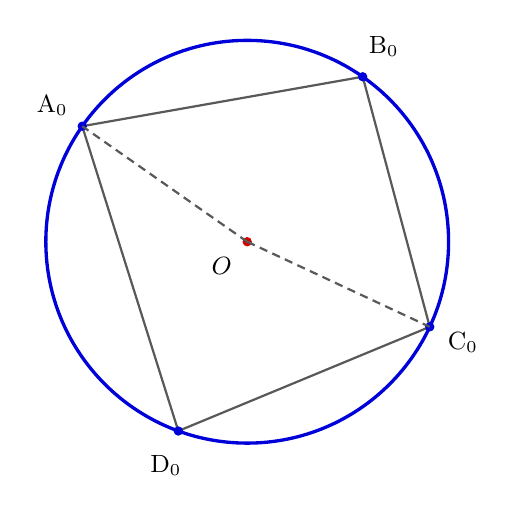
\begin{tikzpicture}[scale=1.55,every node/.style={font=\small}]
      \coordinate (O) at (0,0);
      \coordinate (A) at (145:1.65);
      \coordinate (B) at (55:1.65);
      \coordinate (C) at (-25:1.65);
      \coordinate (D) at (-110:1.65);
      \draw[very thick,blue!85!black] (O) circle (1.65);
      \draw[thick,gray!70!black] (A) -- (B) -- (C) -- (D) -- cycle;
      \foreach \p/\angle in {A/145,B/55,C/-25,D/-110}{
        \node[circle,fill=blue!85!black,inner sep=1.2pt] at (\p) {};
        \node at (\angle:1.95) {$\mathrm{\p}_0$};
      }
      \node[circle,fill=red!85!black,inner sep=1.2pt] at (O) {};
      \node[below left=2pt] at (O) {$O$};
      \draw[densely dashed,thick,gray!70!black] (O) -- (A) (O) -- (C);
    \end{tikzpicture}
    \caption{同一円周上の4点$A_0,B_0,C_0,D_0$}
    \label{1993-3:fig:1}
  \end{figure}
  % TODO :: 誘導に乗るなら，多分$P_nP_n+1が先にあって，その和でQを求める感じだと思う．
  % TODO :: 解答のもっともらしさを述べる
  \newpage
\end{multicols}
\end{document}
